\documentclass{../includes/TechDoc}
\usepackage[T1]{fontenc}
\usepackage[utf8]{inputenc}
%\usepackage[pdftex]{graphicx}
\DeclareGraphicsRule{*}{mps}{*}{}

\title{Мобильное приложение для сообщений о бытовых проблемах студентов в общежитии}
\author{Студент группы БПИ-194}{В. А. Анненков}
\academicTeacher{Доцент департамента программной инженерии факультета компьютерных наук}{Х. М. Салех}

\documentTitle{Пояснительная записка}
\documentCode{RU.17701729.04.03-01 81 01-1-ЛУ}

\begin{document}
    \maketitle

    \begin{abstract}
        В данном программном документе приведена пояснительная записка к мобильному приложению <<Мобильное приложение для сообщений о бытовых проблемах студентов в общежитии>>.

        В данный документ внесены разделы «Введение», «Назначение и область применения программы», «Технические характеристики», «Ожидаемые технико-экономические показатели», «Источники, использованные при разработке».

        В разделе «Введение» указано наименование программы и документы, на основании которых ведется разработка.

        В разделе «Назначение и область применения» указано функциональное назначение программы и эксплуатационное назначение программы.

        В разделе «Технические характеристики» указаны постановка задачи на разработку программы, описание и обоснование метода организации входных и выходных данных, описание и обоснование выбора состава технических и программных средств.

        В разделе «Ожидаемые технико-экономические показатели» указана предполагаемая потребность и экономические преимущества разработки по сравнению с отечественными и зарубежными образцами или аналогами
    \end{abstract}

    \newpage

    \tableofcontents


    \section{Введение}

    \subsection{Наименование программы}

    \subsubsection{Наименование программы на русском языке}

    Мобильное приложение для сообщений о бытовых проблемах студентов в общежитии.

    \subsubsection{Наименование программы на английском языке}

    Mobile Application for Informing about Household Problems in Dormitory.

    \subsection{Основание для разработки}

    Приказ декана факультета компьютерных наук И.В. Аржанцева "Об утверждении тем, руководителей курсовых работ студентов образовательной программы <<Программная инженерия>> факультета компьютерных наук" № 2.3-02/1112-04 от 11.12.2019.


    \section{Назначение и область применения}

    \subsection{Функциональное назначение}

    Функциональным назначением программы является помощь и консультирование студентов по вопросам, связанным
    с проживанием в общежитии. Студент может задать вопрос агенту поддержки, пообщаться в общем чате с другими
    студентами из этого же общежития, узнать последние новости общежития. Агент поддержки имеет доступ к панели
    администрирования, через которую он может создавать объявления, модерировать пользователей и их действия. Отвечать
    на обращения пользователей агент поддержки может с помощью мобильного приложения.

    \subsection{Эксплуатационное назначение}

    Программа может быть использована высшим учебным заведением для обеспечения централизованной связи со студентами, а
    также для информирования студентов о последних новостях в своих общежитиях.


    \section{Технические характеристики}

    \subsection{Постановка задачи}

    Программа должна обеспечивать возможность выполнения следующих функций:

    Для клиента:
    \begin{itemize}[noitemsep]
        \item регистрация и авторизация;
        \item просмотр страницы с новостями;
        \item просмотр и редактирование собственного профиля;
        \item просмотр/создание/удаление/дополнение своих обращений;
        \item просмотр и взаимодействие с общим чатом.
    \end{itemize}

    Для агента поддержки:
    \begin{itemize}[noitemsep]
        \item регистрация и авторизация в приложении;
        \item регистрация и авторизация в панели администрирования;
        \item просмотр и изменение списка новостей;
        \item просмотр/изменение/удаление/дополнение любых обращений.
    \end{itemize}

    Для администратора:
    \begin{itemize}[noitemsep]
        \item всё, что доступно агенту поддержки;
        \item управление существующими агентами поддержки;
        \item возможность назначить или отозвать у пользователя статус агента поддержки;
        \item полный доступ без ограничений к панели администрирования.
    \end{itemize}

    \newpage

    \subsection{Структура облачного хранилища}

    Приведена схема облачного хранилища (Рис.~\ref{fig:api_scheme}).

    В базе данных:
    \begin{itemize}[noitemsep]
        \item таблица auth\_user хранит основную информацию о пользователях;
        \item таблица api\_profile хранит информацию профилей пользователей;
        \item таблица auth\_group хранит пользовательские группы;
        \item таблица auth\_user\_groups хранит группы, к которым принадлежат пользователи;
        \item таблица authtoken\_token хранит токены для авторизации;
        \item таблица auth\_permission хранит информацию о разрешениях;
        \item таблица auth\_group\_permissions хранит разрешения для каждой группы;
        \item таблица auth\_user\_user\_permissions хранит разрешения для каждого пользователя;
        \item таблица api\_dormitory хранит информацию об общежитиях;
        \item таблица api\_problem хранит информацию об обращениях пользователей;
        \item таблица api\_message хранит информацию о сообщениях к обращениям и в общих чатах;
        \item таблица api\_notice хранит информацию о новостях на главной странице;
        \item таблица api\_event хранит информацию о предстоящих событиях.
    \end{itemize}

    \begin{figure}[h]
        \centering
        \frame{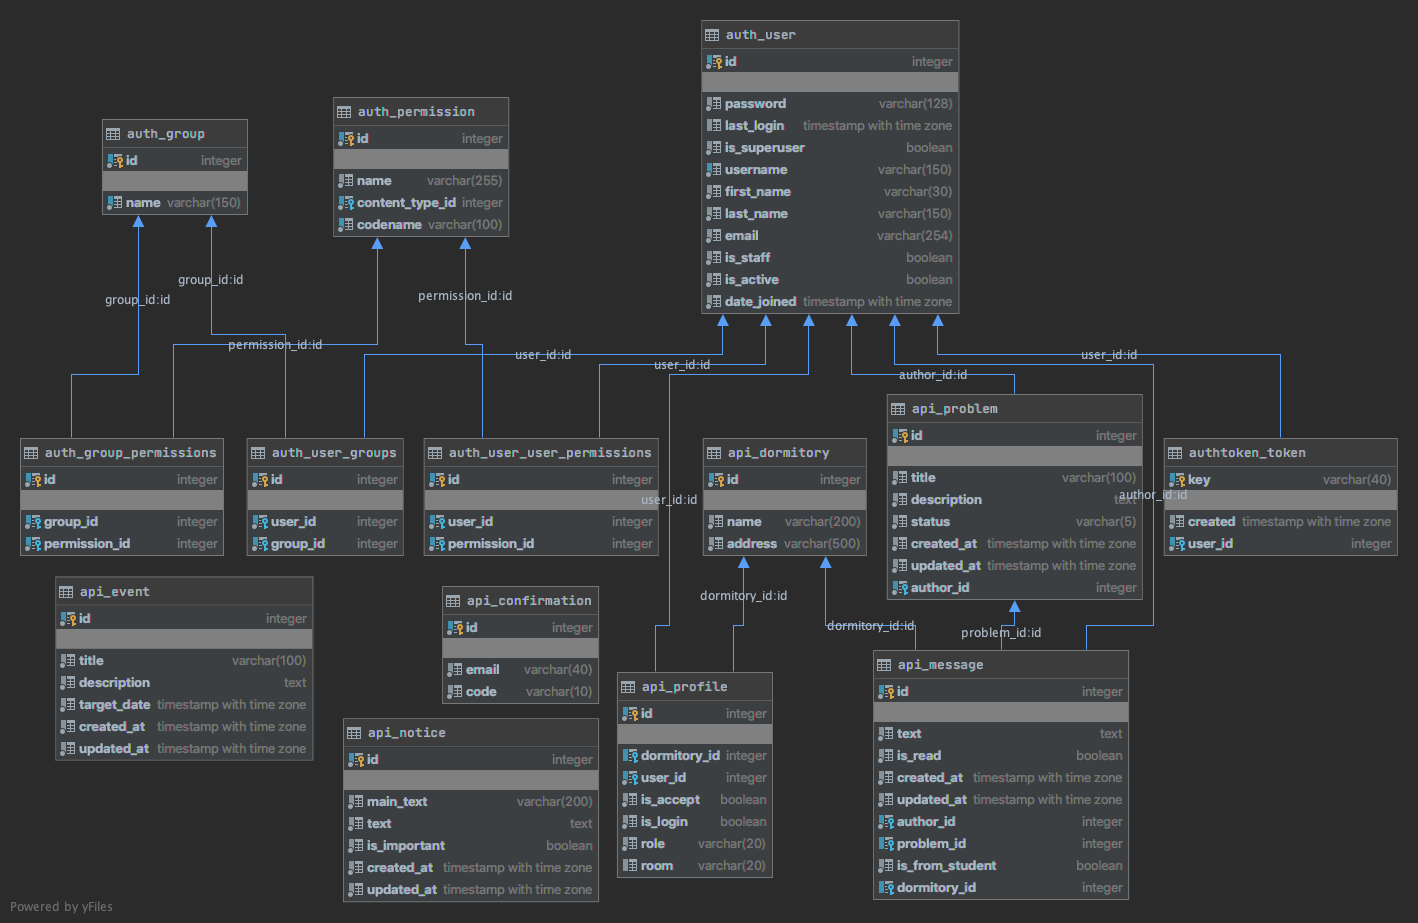
\includegraphics[width=1\linewidth]{images/api_scheme.png}}
        \caption{Схема облачного хранилища}
        \label{fig:api_scheme}
    \end{figure}

    \newpage

    \subsection{Описание алгоритма и функционирования мобильного приложения}

    В мобильном приложении не используются сложные алгоритмы, требующие описания.

    Программа реализована следующим образом:
    \begin{itemize}
        \item пользовательские экраны:
        \begin{itemize}
            \item класс LoginPage представляет собой страницу для авторизации/регистрации пользователя;
            \item класс WaitPage представляет собой форму, которую заполняет новый пользователь после регистрации,
            класс WaitViewModel представляет собой класс с логикой класса WaitPage;
            \item класс MainPage переключает основные пользовательские экраны;
            \item класс MainInfoPage представляет собой главную страницу с новостями и событиями,
            класс MainInfoViewModel представляет собой класс с логикой класса MainInfoPage;
            \item класс ItemsPage представляет собой список обращений пользователя,
            класс WaitViewModel представляет собой класс с логикой класса WaitPage;
            \item класс ItemDetailPage представляет собой страничку отдельного обращения с подробной информацией,
            класс ItemDetailViewModel представляет собой класс с логикой класса ItemDetailPage;
            \item класс ChatPage представляет собой общий чат конкретного общежития,
            класс ChatViewModel представляет собой класс с логикой класса ChatPage;
            \item класс AboutPage представляет собой страницу с описанием приложения,
            класс AboutViewModel представляет собой класс с логикой класса AboutPage;
            \item класс ProfilePage представляет собой форму с данными пользователя с возможностью редактирования,
            класс ProfileViewModel представляет собой класс с логикой класса ProfilePage;
        \end{itemize}
        \item вспомогательные классы:
        \begin{itemize}
            \item класс IHseSupporterApi содержит интерфейсы для взаимодействия с REST API;
            \item класс ApiService хранит необходимые параметры для взаимодействия с REST API;
            \item класс Extensions реализует вспомогательные методы расширения;
        \end{itemize}
        \item классы моделей:
        \begin{itemize}
            \item класс AuthResult содержит информацию об авторизации пользователя;
            \item класс Profile содержит информацию о профиле пользователя.
            \item класс MainPage содержит информацию о наполнении главной страницы;
            \item класс Dormitory содержит информацию об общежитии;
            \item класс Problem содержит информацию об обращении;
            \item класс Message содержит информацию о сообщении в общем чате или к обращению;
            \item класс Notice содержит информацию о новости на главной странице;
            \item класс Event содержит информацию о предстоящем событии;
            \item класс MainQuestion содержит информацию о популярном вопросе;
        \end{itemize}
    \end{itemize}

    \subsection{Описание алгоритма и функционирования сервера}

    На сервере не используются сложные алгоритмы, требующие описания.

    Программа реализована следующим образом:
    \begin{itemize}
        \item REST API классы:
        \begin{itemize}
            \item класс AuthView отправляет защитный код на почту;
            \item класс AuthConfirmView проверяет указанный защитный код с отправленным ранее на почту;
            \item класс ProfileView позволяет получить информацию о своём профиле;
            \item класс MainPageView позволяет получить информацию с главной страницы;
            \item класс DormitoriesViewSet позволяет взаимодействовать с моделями общежитий;
            \item класс ProblemViewSet позволяет взаимодействовать с моделями обращений;
            \item класс MessagesViewSet позволяет взаимодействовать с моделями сообщений;
            \item класс NoticesViewSet позволяет взаимодействовать с моделями новостей;
        \end{itemize}
        \item вспомогательные классы:
        \begin{itemize}
            \item класс IHseSupporterApi содержит интерфейсы для взаимодействия с REST API;
            \item класс ApiService хранит необходимые параметры для взаимодействия с REST API;
            \item класс Extensions реализует вспомогательные методы расширения;
        \end{itemize}
        \item классы моделей:
        \begin{itemize}
            \item класс Profile содержит информацию о профиле пользователя.
            \item класс Dormitory содержит информацию об общежитии;
            \item класс Problem содержит информацию об обращении;
            \item класс Message содержит информацию о сообщении в общем чате или к обращению;
            \item класс Notice содержит информацию о новости на главной странице;
            \item класс Event содержит информацию о предстоящем событии;
            \item класс Confirmation содержит информацию о коде подтверждения;
        \end{itemize}
    \end{itemize}

    \subsection{Описание и обоснование метода организации входных и выходных данных}

    \subsubsection{Для мобильного приложения}

    Входные данные вводятся пользователем вручную в соответствующие для этого текстовые поля или путём нажатия на кнопки интерфейса.

    Выходные данные отображаются в виде текста и иконок.

    \subsubsection{Для сервера}

    Входные данные предоставляются в виде GET/POST/DELETE запросов с дополнительными параметрами.

    Выходные данные предоставляются в виде JSON-модели в качестве ответа на запрос.

    \subsection{Описание и обоснование выбора состава технических и программных средств}

    \subsubsection{Состав технических и программных средств}

    Для работы программы необходим следующий набор программных средств:
    \begin{itemize}
        \item ОС Android 5 или выше.
    \end{itemize}

    Для работы программы необходим следующий набор технических средств:
    \begin{itemize}
        \item стабильное интернет-подключение;
        \item сенсорный экран;
        \item не менее 21 МБ свободной памяти.
    \end{itemize}

    \subsubsection{Обоснование выбора состава технических и программных средств}

    В качестве реализации мобильного приложения были выбраны язык программирования C\# и фреймворк Xamarin.
    Это позволило пользоваться обширной библиотекой пакетов NuGet.

    В качестве реализации серверной части были выбраны язык программирования Python и веб-фреймворк Django.
    Это позволило ускорить процесс разработки за счёт использования вспомогательных библиотек.

    В качестве сервиса для деплоя серверной части был выбран веб-сервис Heroku.
    Это позволило гибко настроить базу данных и подключить автоматический деплой после каждого коммита в ветке master.


    \section{Ожидаемые технико-экономические показатели}

    \subsection{Предполагаемая потребность}

    Мобильное приложение могут использовать образовательные организации для централизованной связи со студентами своих
    общежитий.

    \subsection{Экономические преимущества по сравнению с отечественными и зарубежными аналогами}

    На момент начала разработки на рынке не было выявлено аналогичных продуктов.


    \addition{Описание классов, структур, методов, полей}

    \begin{table}[ht]
        \caption{\label{tab:classes-table}Функциональное назначение классов мобильного приложения.}
        \centering
        \begin{tabular}{ | l | p{12cm} | }
            \hline
            \textbf{Класс} & \textbf{Назначение}  \\ \hline
            LoginPage & Представляет собой страницу для авторизации/регистрации пользователя \\ \hline
            WaitPage & Представляет собой форму, которую заполняет новый пользователь после регистрации \\ \hline
            WaitViewModel & Представляет собой класс с логикой класса WaitPage \\ \hline
            MainPage & Переключает основные пользовательские экраны \\ \hline
            MainInfoPage & Представляет собой главную страницу с новостями и событиями \\ \hline
            MainInfoViewModel & Представляет собой класс с логикой класса MainInfoPage \\ \hline
            ItemsPage & Представляет собой список обращений пользователя \\ \hline
            ItemsViewModel & Представляет собой класс с логикой класса ItemsPage \\ \hline
            ItemDetailPage & Представляет собой страничку отдельного обращения с подробной информацией \\ \hline
            ItemDetailViewModel & Представляет собой класс с логикой класса ItemDetailPage \\ \hline
            ChatPage & Представляет собой общий чат конкретного общежития \\ \hline
            ChatViewModel & Представляет собой класс с логикой класса ChatPage \\ \hline
            AboutPage & Представляет собой страницу с описанием приложения \\ \hline
            AboutViewModel & Представляет собой класс с логикой класса AboutPage \\ \hline
            ProfilePage & Представляет собой форму с данными пользователя с возможностью редактирования \\ \hline
            ProfileViewModel & Представляет собой класс с логикой класса ProfilePage \\ \hline
            IHseSupporterApi & Содержит интерфейсы для взаимодействия с REST API \\ \hline
            ApiService & Хранит необходимые параметры для взаимодействия с REST API \\ \hline
            Extensions & Реализует вспомогательные методы расширения \\ \hline
            Profile & Содержит информацию о профиле пользователя \\ \hline
            Dormitory & Содержит информацию об общежитии \\ \hline
            Problem & Содержит информацию об обращении \\ \hline
            Message & Содержит информацию о сообщении в общем чате или к обращению \\ \hline
            Notice & Содержит информацию о новости на главной странице \\ \hline
            Event & Содержит информацию о предстоящем событии \\ \hline
            Confirmation & Содержит информацию о коде подтверждения \\ \hline
        \end{tabular}
    \end{table}

    \newpage


    \addition{Описание и функциональное назначение полей, методов и свойств}

    \begin{table}[ht]
        \caption{\label{tab:class-loginpage-table}Описание полей, методов и свойств класса LoginPage}
        \centering
        \begin{tabular}{|l|p{3cm}|l|p{3cm}|p{5cm}|}
            \hline
            \multicolumn{5}{|c|}{LoginPage} \\ \hline
            \multicolumn{5}{|l|}{\textbf{Поля}} \\ \hline
            \textbf{Имя} & \textbf{Модификатор доступа} & \textbf{Тип} & \multicolumn{2}{l|}{\textbf{Описание}} \\ \hline
            \_isConfirm & private & bool & \multicolumn{2}{l|}{Подтверждён ли код подтверждения} \\ \hline
            \multicolumn{5}{|l|}{\textbf{Методы}} \\ \hline
            \textbf{Имя} & \textbf{Модификатор доступа} & \textbf{Тип} & \textbf{Аргументы} & \textbf{Назначение} \\ \hline
            LoginPage & public & void & - & Конструктор \\ \hline
            Button\_OnClicked & private & void & object sender, EventArgs e & Выполняет вход при нажатии на кнопку \\ \hline
        \end{tabular}
    \end{table}

    \newpage

    \begin{table}[ht]
        \caption{\label{tab:class-waitpage-table}Описание полей, методов и свойств класса WaitPage}
        \centering
        \begin{tabular}{|l|p{3cm}|l|p{3cm}|p{5cm}|}
            \hline
            \multicolumn{5}{|c|}{WaitPage} \\ \hline
            \multicolumn{5}{|l|}{\textbf{Методы}} \\ \hline
            \textbf{Имя} & \textbf{Модификатор доступа} & \textbf{Тип} & \textbf{Аргументы} & \textbf{Назначение} \\ \hline
            WaitPage & public & void & - & Конструктор \\ \hline
            SaveButton\_OnClicked & private & void & object sender, EventArgs e & Сохраняет введённые данные \\ \hline
        \end{tabular}
    \end{table}

    \newpage

    \begin{table}[ht]
        \caption{\label{tab:class-waitviewmodel-table}Описание полей, методов и свойств класса WaitViewModel}
        \centering
        \begin{tabular}{|l|p{3cm}|l|p{3cm}|p{5cm}|}
            \hline
            \multicolumn{5}{|c|}{WaitViewModel} \\ \hline
            \multicolumn{5}{|l|}{\textbf{Поля}} \\ \hline
            \textbf{Имя} & \textbf{Модификатор доступа} & \textbf{Тип} & \multicolumn{2}{l|}{\textbf{Описание}} \\ \hline
            Dormitories & public & IList & \multicolumn{2}{l|}{Массив общежитий} \\ \hline
            \multicolumn{5}{|l|}{\textbf{Методы}} \\ \hline
            \textbf{Имя} & \textbf{Модификатор доступа} & \textbf{Тип} & \textbf{Аргументы} & \textbf{Назначение} \\ \hline
            WaitViewModel & public & void & - & Конструктор \\ \hline
        \end{tabular}
    \end{table}

    \newpage

    \begin{table}[ht]
        \caption{\label{tab:class-mainpage-table}Описание полей, методов и свойств класса MainPage}
        \centering
        \begin{tabular}{|l|p{3cm}|l|p{3cm}|p{5cm}|}
            \hline
            \multicolumn{5}{|c|}{MainPage} \\ \hline
            \multicolumn{5}{|l|}{\textbf{Методы}} \\ \hline
            \textbf{Имя} & \textbf{Модификатор доступа} & \textbf{Тип} & \textbf{Аргументы} & \textbf{Назначение} \\ \hline
            MainPage & public & void & - & Конструктор \\ \hline
        \end{tabular}
    \end{table}

    \newpage

    \begin{table}[ht]
        \caption{\label{tab:class-maininfopage-table}Описание полей, методов и свойств класса MainInfoPage}
        \centering
        \begin{tabular}{|p{4cm}|p{3cm}|l|p{3cm}|p{5cm}|}
            \hline
            \multicolumn{5}{|c|}{MainInfoPage} \\ \hline
            \multicolumn{5}{|l|}{\textbf{Методы}} \\ \hline
            \textbf{Имя} & \textbf{Модификатор доступа} & \textbf{Тип} & \textbf{Аргументы} & \textbf{Назначение} \\ \hline
            MainInfoPage & public & void & - & Конструктор \\ \hline
            InitProfile & private & void & object sender, EventArgs e & Инициализирует блок с профилем пользователя \\ \hline
            InitMainNotices & private & void & object sender, EventArgs e & Инициализирует блок с главными сообщениями \\ \hline
            InitEvents & private & void & object sender, EventArgs e & Инициализирует блок с событиями \\ \hline
            InitMainQuestions & private & void & object sender, EventArgs e & Инициализирует блок с главными вопросами \\ \hline
            OnError & private & void & object sender, EventArgs e & Отображает ошибку \\ \hline
            MenuItem\_OnClicked & private & void & object sender, EventArgs e & Открывает страницу с профилем \\ \hline
            TapGestureRecognizer \_OnTapped & private & void & object sender, EventArgs e & Открывает подробное описание новости \\ \hline
        \end{tabular}
    \end{table}

    \newpage

    \begin{table}[ht]
        \caption{\label{tab:class-maininfoviewmodel-table}Описание полей, методов и свойств класса MainInfoViewModel}
        \centering
        \begin{tabular}{|p{3.2cm}|p{3cm}|p{3.8cm}|p{3cm}|p{3cm}|}
            \hline
            \multicolumn{5}{|c|}{MainInfoViewModel} \\ \hline
            \multicolumn{5}{|l|}{\textbf{Перечисления}} \\ \hline
            \textbf{Имя} & \textbf{Модификатор доступа} & \multicolumn{3}{p{5cm}|}{\textbf{Описание}} \\ \hline
            ErrorType & public & \multicolumn{3}{l|}{Содержит типы ошибки} \\ \hline
            \multicolumn{5}{|l|}{\textbf{Свойства}} \\ \hline
            \textbf{Имя} & \textbf{Модификатор доступа} & \textbf{Тип} & \multicolumn{2}{p{6.8cm}|}{\textbf{Описание}} \\ \hline
            RefreshCommand & public & Command & \multicolumn{2}{p{6.8cm}|}{Хранит действие, которое воспроизводится при свайпе вверх} \\ \hline
            Profile & public & Profile & \multicolumn{2}{p{6.8cm}|}{Хранит загруженный профиль} \\ \hline
            AllNotices & public & List<Notice> & \multicolumn{2}{p{6.8cm}|}{Хранит загруженные новости} \\ \hline
            Notices & public & ObservableCollection <Notice> & \multicolumn{2}{p{6.8cm}|}{Хранит загруженные новости с фильтром "не важное"} \\ \hline
            Events & public & ObservableCollection <Event> & \multicolumn{2}{p{6.8cm}|}{Хранит загруженные предстоящие события} \\ \hline
            MainQuestions & public & ObservableCollection <MainQuestion> & \multicolumn{2}{p{6.8cm}|}{Хранит загруженные популярные вопросы} \\ \hline
            \multicolumn{5}{|l|}{\textbf{События}} \\ \hline
            \textbf{Имя} & \textbf{Модификатор доступа} & \textbf{Тип} & \multicolumn{2}{p{6.8cm}|}{\textbf{Описание}} \\ \hline
            Load & public & EventHandler & \multicolumn{2}{p{6.8cm}|}{Событие, которое вызывается при успешной загрузке} \\ \hline
            Error & public & EventHandler & \multicolumn{2}{p{6.8cm}|}{Событие, которое вызывается при ошибке} \\ \hline
            \multicolumn{5}{|l|}{\textbf{Методы}} \\ \hline
            \textbf{Имя} & \textbf{Модификатор доступа} & \textbf{Тип} & \textbf{Аргументы} & \textbf{Назначение} \\ \hline
            MainInfoView Model & public & void & - & Конструктор \\ \hline
            InitMainPage & public & void & - & Загружает информацию о главной странице с сервера \\ \hline
            OnLoad & public & void & - & Вызывается после успешной загрузки, вызывает метод отрисовки загруженной информации \\ \hline
            OnError & public & void & - & Вызывается после неуспешной загрузки \\ \hline
        \end{tabular}
    \end{table}

    \newpage

    \begin{table}[ht]
        \caption{\label{tab:class-profilepage-table}Описание полей, методов и свойств класса ProfilePage}
        \centering
        \begin{tabular}{|p{3.2cm}|p{3cm}|p{3.8cm}|p{3cm}|p{3cm}|}
            \hline
            \multicolumn{5}{|c|}{ProfilePage} \\ \hline
            \multicolumn{5}{|l|}{\textbf{Методы}} \\ \hline
            \textbf{Имя} & \textbf{Модификатор доступа} & \textbf{Тип} & \textbf{Аргументы} & \textbf{Назначение} \\ \hline
            ProfilePage & public & void & - & Конструктор \\ \hline
            SaveButton \_OnClicked & private & void & object sender, EventArgs e & Сохраняет данные \\ \hline
        \end{tabular}
    \end{table}

    \newpage

    \begin{table}[ht]
        \caption{\label{tab:class-profileviewmodel-table}Описание полей, методов и свойств класса ProfileViewModel}
        \centering
        \begin{tabular}{|p{3.2cm}|p{3cm}|p{3.8cm}|p{3cm}|p{3cm}|}
            \hline
            \multicolumn{5}{|c|}{ProfileViewModel} \\ \hline
            \multicolumn{5}{|l|}{\textbf{Поля}} \\ \hline
            \textbf{Имя} & \textbf{Модификатор доступа} & \textbf{Тип} & \multicolumn{2}{l|}{\textbf{Описание}} \\ \hline
            Dormitories & public & IList & \multicolumn{2}{l|}{Массив общежитий} \\ \hline
            \multicolumn{5}{|l|}{\textbf{Свойства}} \\ \hline
            \textbf{Имя} & \textbf{Модификатор доступа} & \textbf{Тип} & \multicolumn{2}{l|}{\textbf{Описание}} \\ \hline
            FirstName & public & string & \multicolumn{2}{l|}{Имя пользователя} \\ \hline
            LastName & public & string & \multicolumn{2}{l|}{Фамилия пользователя} \\ \hline
            Room & public & string & \multicolumn{2}{l|}{Комната пользователя} \\ \hline
            \multicolumn{5}{|l|}{\textbf{Методы}} \\ \hline
            \textbf{Имя} & \textbf{Модификатор доступа} & \textbf{Тип} & \textbf{Аргументы} & \textbf{Назначение} \\ \hline
            ProfileViewModel & public & void & - & Конструктор \\ \hline
        \end{tabular}
    \end{table}

    \newpage

    \begin{table}[ht]
        \caption{\label{tab:class-itemspage-table}Описание полей, методов и свойств класса ItemsPage}
        \centering
        \begin{tabular}{|l|p{3cm}|l|p{3cm}|p{3cm}|}
            \hline
            \multicolumn{5}{|c|}{ItemsPage} \\ \hline
            \multicolumn{5}{|l|}{\textbf{Поля}} \\ \hline
            \textbf{Имя} & \textbf{Модификатор доступа} & \textbf{Тип} & \multicolumn{2}{l|}{\textbf{Описание}} \\ \hline
            \_viewModel & private & ItemsViewModel & \multicolumn{2}{l|}{Экземпляр класса с логикой экрана} \\ \hline
            \multicolumn{5}{|l|}{\textbf{Методы}} \\ \hline
            \textbf{Имя} & \textbf{Модификатор доступа} & \textbf{Тип} & \textbf{Аргументы} & \textbf{Назначение} \\ \hline
            ItemsPage & public & void & - & Конструктор \\ \hline
            OnItemSelected & private & void & object sender, SelectedItem ChangedEvent Args args & Открывает страницу с детальной информацией об обращении \\ \hline
            OnAppearing & protected & void & - & Вызывается при отнрытии страницы, обновляет список обращений \\ \hline
            MenuItem\_OnDelete & private & void & object sender, EventArgs e & Удаляет обращение \\ \hline
        \end{tabular}
    \end{table}

    \newpage

    \begin{table}[ht]
        \caption{\label{tab:class-itemdetailpage-table}Описание полей, методов и свойств класса ItemDetailPage}
        \centering
        \begin{tabular}{|p{2.9cm}|p{3cm}|p{2cm}|p{3cm}|p{5cm}|}
            \hline
            \multicolumn{5}{|c|}{ItemDetailPage} \\ \hline
            \multicolumn{5}{|l|}{\textbf{Поля}} \\ \hline
            \textbf{Имя} & \textbf{Модификатор доступа} & \textbf{Тип} & \multicolumn{2}{l|}{\textbf{Описание}} \\ \hline
            \_viewModel & private & ItemDetail ViewModel & \multicolumn{2}{l|}{Экземпляр класса с логикой экрана} \\ \hline
            \multicolumn{5}{|l|}{\textbf{Методы}} \\ \hline
            \textbf{Имя} & \textbf{Модификатор доступа} & \textbf{Тип} & \textbf{Аргументы} & \textbf{Назначение} \\ \hline
            ItemDetailPage & public & void & - & Конструктор \\ \hline
            ItemDetailPage & public & void & ItemDetail ViewModel viewModel & Конструктор \\ \hline
            InitItem & private & void & object sender, EventArgs e & Инициализирует страницу обращения \\ \hline
            SendButton \_OnClicked & private & void & object sender, EventArgs e & Отправляет сообщение в обращении \\ \hline
        \end{tabular}
    \end{table}

    \newpage

    \begin{table}[ht]
        \caption{\label{tab:class-chatpage-table}Описание полей, методов и свойств класса ChatPage}
        \centering
        \begin{tabular}{|l|p{3cm}|p{2cm}|p{3cm}|p{3cm}|}
            \hline
            \multicolumn{5}{|c|}{ChatPage} \\ \hline
            \multicolumn{5}{|l|}{\textbf{Поля}} \\ \hline
            \textbf{Имя} & \textbf{Модификатор доступа} & \textbf{Тип} & \multicolumn{2}{l|}{\textbf{Описание}} \\ \hline
            \_viewModel & private & ChatView Model & \multicolumn{2}{l|}{Экземпляр класса с логикой экрана} \\ \hline
            \multicolumn{5}{|l|}{\textbf{Методы}} \\ \hline
            \textbf{Имя} & \textbf{Модификатор доступа} & \textbf{Тип} & \textbf{Аргументы} & \textbf{Назначение} \\ \hline
            ChatPage & public & void & - & Конструктор \\ \hline
            ChatPage & public & void & ChatViewModel viewModel & Конструктор \\ \hline
            InitChat & private & Task & bool isScrollDown & Инициализирует список сообщений \\ \hline
            SendButton\_OnClicked & private & void & object sender, EventArgs e & Отправляет сообщение в чат \\ \hline
        \end{tabular}
    \end{table}

    \newpage

    \begin{table}[ht]
        \caption{\label{tab:class-aboutpage-table}Описание полей, методов и свойств класса AboutPage}
        \centering
        \begin{tabular}{|l|l|l|l|l|}
            \hline
            \multicolumn{5}{|c|}{AboutPage} \\ \hline
            \multicolumn{5}{|l|}{\textbf{Методы}} \\ \hline
            \textbf{Имя} & \textbf{Модификатор доступа} & \textbf{Тип} & \textbf{Аргументы} & \textbf{Назначение} \\ \hline
            AboutPage & public & void & - & Конструктор \\ \hline
        \end{tabular}
    \end{table}

    \newpage

    \begin{table}[ht]
        \caption{\label{tab:class-ihsesupporterapi-table}Описание полей, методов и свойств класса IHseSupporterApi}
        \centering
        \begin{tabular}{|l|p{3cm}|p{3.7cm}|p{3.4cm}|p{3.5cm}|}
            \hline
            \multicolumn{5}{|c|}{IHseSupporterApi} \\ \hline
            \multicolumn{5}{|l|}{\textbf{Методы}} \\ \hline
            \textbf{Имя} & \textbf{Модификатор доступа} & \textbf{Тип} & \textbf{Аргументы} & \textbf{Назначение} \\ \hline
            Login & - & Task<AuthResult> & Dictionary<string, object> data & Отправляет запрос на получение защитного кода \\ \hline
            LoginConfirm & - & Task<AuthResult> & Dictionary<string, object> data & Подтверждает авторизацию \\ \hline
            GetMainPage & - & Task<MainPage> & - & Получает информацию на главной странице \\ \hline
            SetProfile & - & Task<Profile> & Dictionary<string, object> data & Обновляет информацию профиля пользователя \\ \hline
            GetDormitory & - & Task<Dormitory> & int id & Получает информацию об общежитии \\ \hline
            GetProblems & - & Task<List <Problem> > & - & Получает список обращений \\ \hline
            SaveProblem & - & Task<Problem> & - & Сохраняет информацию об обращении \\ \hline
            GetProblem & - & Task<Problem> & int id & Получает информацию о проблеме \\ \hline
            DeleteProblem & - & Task<Problem> & int id & Удаляет проблему \\ \hline
            SendMessage & - & Task<Message> & Dictionary<string, object> data & Отправляет сообщение \\ \hline
        \end{tabular}
    \end{table}

    \newpage

    \begin{table}[ht]
        \caption{\label{tab:class-apiservice-table}Описание полей, методов и свойств класса ApiService}
        \centering
        \begin{tabular}{|l|p{3cm}|p{3.3cm}|p{2.4cm}|l|}
            \hline
            \multicolumn{5}{|c|}{ApiService} \\ \hline
            \multicolumn{5}{|l|}{\textbf{Поля}} \\ \hline
            \textbf{Имя} & \textbf{Модификатор доступа} & \textbf{Тип} & \multicolumn{2}{l|}{\textbf{Описание}} \\ \hline
            HseSupporterApi & public & IHseSupporterApi & \multicolumn{2}{p{7cm}|}{Экземпляр класса с REST API методами} \\ \hline
            TokenHeader & public & string & \multicolumn{2}{l|}{Хранит header запросов} \\ \hline
            \multicolumn{5}{|l|}{\textbf{Методы}} \\ \hline
            \textbf{Имя} & \textbf{Модификатор доступа} & \textbf{Тип} & \textbf{Аргументы} & \textbf{Назначение} \\ \hline
            ApiService & public & - & - & Конструктор \\ \hline
        \end{tabular}
    \end{table}

    \newpage

    \begin{table}[ht]
        \caption{\label{tab:class-extensions-table}Описание полей, методов и свойств класса Extensions}
        \centering
        \begin{tabular}{|l|p{3cm}|l|p{3cm}|p{5cm}|}
            \hline
            \multicolumn{5}{|c|}{Extensions} \\ \hline
            \multicolumn{5}{|l|}{\textbf{Методы}} \\ \hline
            \textbf{Имя} & \textbf{Модификатор доступа} & \textbf{Тип} & \textbf{Аргументы} & \textbf{Назначение} \\ \hline
            GetDateTimeText & public & string & this string str & Преобразует строку с датой в читаемый вид \\ \hline
        \end{tabular}
    \end{table}

    \newpage


    \begin{thebibliography}{3}
        \bibitem{gost}Единая система программной документации – М.: ИПК, Издательство стандартов, 2000, 125 стр.
        \bibitem{lms} LMS [Электронный ресурс] URL: \url{https://lms.hse.ru/} (Дата обращения: 30.04.2020, режим доступа: свободный)
        \bibitem{ruz} РУЗ [Электронный ресурс] URL: \url{https://ruz.hse.ru/} (Дата обращения: 30.04.2020, режим доступа: свободный)
        \bibitem{github} GitHub [Электронный ресурс] URL: \url{https://github.com/} (Дата обращения: 30.04.2020, режим доступа: свободный)
        \bibitem{microsoft} Документация Microsoft [Электронный справочник] URL: \url{https://docs.microsoft.com/ru-ru/} (Дата обращения: 30.04.2020, режим доступа: свободный)
        \bibitem{stackoverflow} StackOverflow [Электронный ресурс] URL: \url{https://stackoverflow.com/} (Дата обращения: 30.04.2020, режим доступа: свободный)
    \end{thebibliography}


    \registrationList

\end{document}
